\documentclass{report}

\usepackage{fontspec}
\setmainfont{Inconsolata}

\usepackage[hidelinks,unicode,bookmarks=true]{hyperref}
\usepackage{fancyvrb}
\usepackage{color}
\usepackage{graphicx}
\usepackage{amsmath}
\usepackage{amsthm}
\usepackage{amssymb}
%\usepackage{relsize}
\usepackage{centernot}
\usepackage[top=3cm, left=3cm, right=3cm, bottom=2cm]{geometry}
\usepackage{titling}
%\usepackage{lipsum}
\usepackage{standalone}
\usepackage{enumitem}

\usepackage{ulem}

\setlength{\droptitle}{-3em}

\newtheoremstyle{break}
{\topsep}{\topsep}%
{\itshape}{}%
{\bfseries}{}%
{\newline}{}%
\theoremstyle{break}
\newtheorem{defn}{Definition}
\newtheorem{thm}{Theorem}
\newtheorem*{coro}{Corollary}
\newtheorem{lemma}{Lemma}
\newtheorem*{remark}{Remark}
\newtheorem*{note}{Note}
\newtheorem*{prob}{Problem}
\newtheorem*{soln}{Solution}
\newtheorem*{claim}{Claim}
\renewcommand*{\proofname}{Proof}

\title{
	The Incomplete Codex of Basic Mathematics for Computer Scientists\\
	\large From Programmers to Hackers: Mathematical Basis to Computer Science
}

\author{None(\href{https://www.twitter.com/n0n3x1573n7}{@n0n3x1573n7})}

\date{\today}

\begin{document}
	\maketitle

	\chapter{Introduction}
		\documentclass{report}

\begin{document}
\end{document}
	
	\tableofcontents
	
	\part{Mathematical Preliminaries}
	
		\chapter{Algebraic Structures}
			\documentclass{report}

\begin{document}

	\section{Algebraic Structures}

		\subsection{Sets}

			\begin{defn}[Set] \label{def_set}
				A \emph{set} is a collection of distinct objects. 
			\end{defn}
		
			To see some traits on sets, we literally start from nothing:
			\begin{axiom}[Empty Set Axiom] \label{axiom_empty_set}
				There is a set containing no members, that is:
				\begin{displaymath}
				\exists B \text{ such that } \forall x, (x \notin B)
				\end{displaymath}
				We call this set the \emph{empty set}, and denote it by the symbol $\emptyset$.
			\end{axiom}

			We now have $\emptyset$; we now write down a few rules for how to manipulate sets.
			\begin{axiom}[Axiom of Extensionality] \label{axiom_extensionality}
				Two sets are equal if and only if they share the same elements, that is:
				\begin{displaymath}
				\forall A,B [\forall z,((z \in A) \Leftrightarrow (z \in B)) \Rightarrow (A=B)]
				\end{displaymath}
			\end{axiom}

			\begin{axiom}[Axiom of Pairing] \label{axiom_pairing}
				Given any two sets $A$ and $B$, there is a set which have the members just $A$ and $B$, that is:
				\begin{displaymath}
					\forall A,B \exists C \forall x [x \in C \Leftrightarrow ((x=A) \vee (x=B))]
				\end{displaymath}
				If $A$ and $B$ are distinct sets, we write this set $C$ as $\{A,B\}$; if $A=B$, we write it as $\{A\}$.
			\end{axiom}
	
			\begin{axiom}[Axiom of Union, simple version] \label{axiom_union_simple}
				Given any two sets $A$ and $B$, there is a set whose members are those sets belonging to either $A$ or $B$, that is:
				\begin{displaymath}
					\forall A,B \exists C \forall x [x \in C \Leftrightarrow ((x \in A) \vee (x \in B))]
				\end{displaymath}
				We write this set $C$ as $A \cup B$.
			\end{axiom}
			
			In the simplified version of Axiom of Union, we take union of only two things, but we sometimes we want to take unions of more than two things or even more than finitely many things. This is given by the full version of the axiom:
		
			\begin{axiom}[Axiom of Union, full version] \label{axiom_union_full}
				Given any set $A$, there is a set $C$ whose elements are exactly the members of the members of $A$, that is:
				\begin{displaymath}
					\forall A \exists C [x \in C \Leftrightarrow (\exists A'(A' \in A) \wedge (x \in A'))]
				\end{displaymath}
				We denote this set $C$ as
				\begin{displaymath}
					\bigcup_{A' \in A}A'
				\end{displaymath}
			\end{axiom}

			\begin{axiom}[Axiom of Intersection, simple version] \label{axiom_intersection_simple}
				Given any two sets $A$ and $B$, there is a set whose members are member of both $A$ and $B$, that is:
				\begin{displaymath}
					\forall A,B \exists C \forall x [(x \in C) \Leftrightarrow ((x \in A ) \wedge (x \in B))]
				\end{displaymath}
			\end{axiom}
	
			Sometimes as union, we would want to take intersection of more than finitely many things. This is given by the full version of the axiom:
			
			\begin{axiom}[Axiom of Intersection, full version] \label{axiom_intersection_full}
				Given any set $A$, there is a set $C$ whose elements are exactly the members of all members of $A$, that is:
				\begin{displaymath}
					\forall A \exists C \forall x [(x \in C) \Leftrightarrow (\forall A'((A' \in A) \Rightarrow (x \in A')))]
				\end{displaymath}
				We denote this set $C$ as
				\begin{displaymath}
					\bigcap_{A' \in A}A'
				\end{displaymath}
			\end{axiom}
		
			\begin{axiom}[Axiom of Subset] \label{axiom_subset}
				For any two sets $A$ and $B$, we say that $B \subset A$ if and only if every member of B is a member of A, that is:
				\begin{displaymath}
					(B \subseteq A) \Leftrightarrow (\forall x (x \in B) \Rightarrow (x \in A))
				\end{displaymath}
			\end{axiom}
			
			By the Axiom of Subset we can define the power set of an any given set:
			
			\begin{defn}[Power Set] \label{def_powerset}
				For any set $A$, the \emph{power set} of the set $A$, denoted $P(A)$, whose members are precisely the collection of all possible subsets of A, that is:
				\begin{displaymath}
					\forall A \exists P(A) \forall B((B \subseteq A) \Leftrightarrow (B \in P(A)))
				\end{displaymath}
			\end{defn}

			\begin{defn}[Order] \label{def_order}
				Let $S$ be a set. An \emph{order} on $S$ is a relation, denoted by $<$, with the following properties:
				\begin{itemize}
					\item If $x \in S$ and $y \in S$ then one and only one of the following statements is true:
					\begin{displaymath}
						x<y, x=y, y<x
					\end{displaymath}
					\item For $x,y,z \in S$, if $x<y$ and $y<z$, then $x<z$.
				\end{itemize}
			\end{defn}

			\begin{remark} \label{remark_order}
				\begin{itemize}
					\item[]
					\item It is possible to write $x>y$ in place of $y<x$
					\item The notation $x \leq y$ indicates that $x<y$ or $x=y$.
				\end{itemize}
			\end{remark}

		\begin{defn}[Ordered Set] \label{def_ordered_set}
			An \emph{ordered set} is a set in which an order is defined.
		\end{defn}

		\begin{defn}[Bound] \label{def_bound}
			Suppose $S$ is an ordered set, and $E\subset S$.\\
			If there exists $\beta \in S$ such that $x \leq \beta$ for every $x \in E$, we say that E is \emph{bounded above}, and call $\beta$ an \emph{upper bound} of E.
			If there exists $\alpha \in S$ such that $x \geq \alpha$ for every $x \in E$, we say that E is \emph{bounded below}, and call $\alpha$ a \emph{lower bound} of E.
		\end{defn}

		\begin{defn}[Least Upper Bound] \label{def_supremum}
			Suppose that $S$ is an ordered set, and $E \subset S$.
			If there exists a $\beta \in S$ with the following properties:
			\begin{itemize}
				\item $\beta$ is an upper bound of $E$
				\item If $\gamma < \beta$, then $\gamma$ is not an upper bound of E
			\end{itemize}
			Then $\beta$ is called the \emph{Least Upper Bound} of E or the \emph{supremum} of E, denoted
			\begin{displaymath}
				\beta=sup(E)
			\end{displaymath}
		\end{defn}

		\begin{defn}[Greatest Lower Bound] \label{def_infimum}
			Suppose that $S$ is an ordered set, and $E \subset S$.
			If there exists a $\alpha \in S$ with the following properties:
			\begin{itemize}
				\item $\alpha$ is a lower bound of $E$
				\item If $\gamma < \alpha$, then $\gamma$ is not an lower bound of E
			\end{itemize}
			Then $\alpha$ is called the \emph{Greatest Lower Bound} of E or the \emph{infimum} of E, denoted
			\begin{displaymath}
			\beta=inf(E)
			\end{displaymath}
		\end{defn}

		\begin{defn}[least-upper-bound property] \label{def_least_upper_bound_property}
			An ordered set $S$ is said to have the \emph{least-upper-bound property} if the following is true:\\
			if $E \subset S$, $E$ is not empty, and $E$ is bounded above, then $sup(E)$ exists in $S$.
		\end{defn}

		\begin{defn}[greatest-lower-bound property] \label{def_greatest_lower_bound_property}
			An ordered set $S$ is said to have the \emph{greatest-lower-bound property} if the following is true:\\
			if $E \subset S$, $E$ is not empty, and $E$ is bounded below, then $inf(E)$ exists in $S$.
		\end{defn}

		\begin{thm} \label{thm_glb_lub_property}
			Suppose $S$ is an ordered set with the least-upper-bound property, $B \subset S$, $B$ is not empty, and $B$ is bounded below.\\
			Let $L$ be the set of all lower bounds of $B$. Then
			\begin{displaymath}
				\alpha=sup(L)
			\end{displaymath}
			exists in $S$, and $\alpha=inf(B)$.
		\end{thm}

		\begin{proof}
			Note that $\forall x \in L, y \in B, x \leq y$.\\
			$L$ is nonempty as $B$ is bounded below.\\
			$L$ is bounded above since $\forall x \in S \backslash L, \forall y \in L, x>y$.\\
			Since $S$ has the least-upper-bound property and $L \subset S$, $\exists \alpha=sup(L)$.\\
			The followings hold:
			\begin{itemize}
				\item $\alpha$ is a lower bound of $B$.
					\\($\because$) $\forall \gamma \in B, \gamma > \alpha$
				\item $\beta$ with $\beta > \alpha$ is not a lower bound of $B$
					\\($\because$)Since $\alpha$ is an upper bound of $L$, $\beta \notin L$.
			\end{itemize}
			Hence $\alpha=inf(B)$.
		\end{proof}
		
		\begin{coro} \label{coro_glb_lub_property_equiv}
			For all ordered sets, the Least Upper Bound property and the Greatest Lower Bound Porperty are equivalent.
		\end{coro}

		\subsection{Group}

			\begin{defn}[Group] \label{def_group}
				A \emph{group} is a set $G$ with a binary operation $\cdot$, denoted $(G,\cdot)$, which satisfies the following conditions:
				\begin{itemize}
					\item \textbf{Closure}: $\forall a,b \in G, a \cdot b \in G$
					\item \textbf{Associativity}: $\forall a,b,c \in G, (a \cdot b) \cdot c=a \cdot (b \cdot c)$
					\item \textbf{Identity}: $\exists e \in G, \forall a \in G, a \cdot e=e \cdot a=a$
					\item \textbf{Inverse}: $\forall a \in G, \exists a^{-1} \in G, a \cdot a^{-1}=a^{-1} \cdot a=e$
				\end{itemize}
			\end{defn}

		\begin{defn}[Semigroup] \label{def_semigroup}
			A \emph{semigroup} is $(G,\cdot)$, which satisfies Closure and Associativity.
		\end{defn}

		\begin{defn}[Monoid] \label{def_monoid}
			A \emph{monoid} is a semigroup $(G,\cdot)$ which also has identity.
		\end{defn}

		\begin{defn}[Abelian Group] \label{def_abelian_group}
			An \emph{Abelian Group} or \emph{Commutative Group} is a group $(G,\cdot)$ with the following property:
			\begin{itemize}
				\item \textbf{Commutativity}: $\forall a,b \in G, a \cdot b=b \cdot a$
			\end{itemize}
		\end{defn}

		\subsection{Ring}

			\begin{defn}[Ring] \label{def_ring}
				A \emph{Ring} is a set $R$ with two binary operations $+$ and $\cdot$, often called the addition and multiplication of the ring, denoted $(R,+,\cdot)$, which satisfies the following conditions:
				\begin{itemize}
					\item $(R,+)$ is an abelian group
					\item $(R,\cdot)$ is a semigroup
					\item \textbf{Distribution}: $\cdot$ is distributive with respect to $+$, that is, $\forall a,b,c \in R$:
					\begin{itemize}[label=-]
						\item $a \cdot (b + c)=(a \cdot b) + (a \cdot c)$
						\item $(a + b) \cdot c=(a \cdot c) + (b \cdot c)$
					\end{itemize}
				\end{itemize}
			The identity element of $+$ is often noted $0$.
			\end{defn}

		\begin{defn}[Ring with identity(1)] \label{def_ring_with_1}
			A \emph{Ring with identity} is a ring $(R,+,\cdot)$ of which $(R,\cdot)$ is a monoid. The identity element of $\cdot$ is often noted $1$.
		\end{defn}

		\begin{defn}[Commutative Ring] \label{def_commutative_ring}
			A \emph{commutative ring} is a ring $(R,+,\cdot)$ of which $\cdot$ is commutative.
		\end{defn}

		\begin{defn}[Zero Divisor] \label{def_zero_divisor}
			For a ring $(R,+,\cdot)$, let $0$ be the identity of $+$.\\
			$a,b\in R$, $a \neq 0$ and $b \neq 0$, if $a \cdot b=0$, $a,b$ are called the zero divisors of the ring.
		\end{defn}

		\begin{defn}[Integral Domain] \label{def_integral_domain}
			An \emph{integral domain} is a commutative ring $(R,+,\cdot)$ with 1 which does not have zero divisors.
		\end{defn}

		\subsection{Field}

		\begin{defn}[Field] \label{def_field}
			A \emph{Field} is a set $F$ with two binary operations $+$ and $\cdot$, often called the addition and multiplication of the field, denoted $(R,+,\cdot)$, which satisfies the following conditions:
			\begin{itemize}
				\item $(F,+,\cdot)$ is a ring
				\item $(F\backslash \{0\},\cdot)$ is a group
			\end{itemize}
			Alternatively, a Field may be defined with a set of \emph{Field Axioms} listed below:
			\begin{itemize}
					\item[(A)] \textbf{Axioms for Addition}
					\begin{itemize}
						\item[(A1)] \textbf{Closed under Addition}\\$\forall a,b \in F, a+b \in F$
						\item[(A2)] \textbf{Addition is Commutative}\\$\forall a,b \in F, a+b=b+a$
						\item[(A3)] \textbf{Addition is Associative}\\$\forall a,b,c \in F, (a+b)+c=a+(b+c)$
						\item[(A4)] \textbf{Identity of Addition}\\$\exists 0 \in F, \forall a \in F, 0+a=a$
						\item[(A5)] \textbf{Inverse of Addition}\\$\forall a \in F, \exists -a \in F, a+(-a)=0$
					\end{itemize}
					\item[(M)] \textbf{Axioms for Multiplication}
					\begin{itemize}
						\item[(M1)] \textbf{Closed under Multiplication}\\$\forall a,b \in F, a \cdot b \in F$
						\item[(M2)] \textbf{Multiplication is Commutative}\\$\forall a,b \in F, a \cdot b=b \cdot a$
						\item[(M3)] \textbf{Multiplication is Associative}\\$\forall a,b,c \in F, (a \cdot b) \cdot c=a \cdot (b \cdot c)$
						\item[(M4)] \textbf{Identity of Multiplication}\\$\exists 1 \in F, \forall a \in F, 1 \cdot a=a$
						\item[(M5)] \textbf{Inverse of Multiplication}\\$\forall a \in F\backslash\{0\}, \exists a^{-1} \in F, a \cdot a^{-1}=1$
					\end{itemize}
				\item[(D)] \textbf{Distributive Law}
				\\$\forall a,b,c \in F, (a+b) \cdot c=a \cdot c+b \cdot c$\\where $\cdot$ takes precedence over $+$.
			\end{itemize}
		\end{defn}

		\begin{defn}[Ordered Field] \label{def_ordered_field}
			An \emph{ordered field} is a field $F$ which is an ordered set, such that
			\begin{itemize}
				\item $x+y<x+z$ if $x,y,z \in F$ and $y<z$
				\item $xy>0$ if $x,y \in F$, $x>0$ and $y>0$
			\end{itemize}
			\end{defn}

		\begin{thm}[Existence of $\mathbb{R}$] \label{thm_existence_real_number}
			There exists an ordered field $\mathbb{R}$ containing $\mathbb{Q}$ as a subfield which has the least-upper-bound property.
		\end{thm}

		\begin{defn}[Extended Real Number System] \label{def_extended_real_number_system}
			The \emph{extended real number system}, denoted $\overline{\mathbb{R}}$, $[-\infty,\infty]$, or $\mathbb{R} \cup \{-\infty,\infty\}$, consists of the real field $\mathbb{R}$ and two symbols, $+\infty$ and $-\infty$. We preserve the original order in $\mathbb{R}$, and define $\forall x \in \mathbb{R}$,
			\begin{displaymath}
				-\infty<x<\infty
			\end{displaymath}
		\end{defn}

		\begin{remark} \label{remark_extended_real_number_system_not_field}
			The extended real number system does not form a field.
		\end{remark}
	
		\subsection{Polynomial Ring}
		\begin{defn}[Polynomial over a Ring] \label{def_polynomial}
			A polynomial $f(x)$ over the ring $(R,+,\cdot)$ is defined as
			\begin{displaymath}
				f(x)=\sum_{i=0}^{\infty}a_ix^i=a_0+a_1x^1+\cdots,a_i\in R
			\end{displaymath}
			where $a_i=0$ for all but finitely many values of $i$.\\
			The \emph{degree} of the polynomial $\deg(f)$ is defined as $\deg(f)=\max\{n|n\in\mathbb{N}, a_n\ne0 \}$.
			The \emph{leading coefficient} of the polynomial is defined as $a_{\deg(f)}$.
		\end{defn}

		\begin{defn}[Addition and Multiplication of Polynomials] \label{def_add_mult_polynomial}
			Let $f(x)=\sum_{i=0}^{\infty}a_ix^i$, $g(x)=\sum_{i=0}^{\infty}b_ix^i$, $a_i,b_i \in R$ be a polynomial over the ring $(R,+,\cdot)$. Define:
			\begin{gather*}
				f(x)+g(x)=\sum_{i=0}^{\infty}(a_i+b_i)x^i\\
				f(x)g(x)=\sum_{k=0}^{\infty}(c_k)x^k \text{ where } c_k=\sum_{i+j=k}a_ib_j
			\end{gather*}
		\end{defn}

		\begin{defn}[Polynomial Ring] \label{def_polynomial_ring}
			The set of polynomials over the ring $(R,+,\cdot)$, $R[x]=\{f(x)|f(x) \text{ is a polynomial over } R \}$ is called the \emph{Polynomial Ring(or Polynomials) over $R$}.
		\end{defn}

		\begin{thm}[Degree of Polynomial on Addition and Multiplication] \label{thm_add_mult_deg}
			Let $f(x),g(x) \in R[x]$ with $\deg(f)=n$, $\deg(g)=m$.
			\begin{itemize}
				\item $0 \le \deg(f+g) \le \max(\deg(f),\deg(g))$
				\item $\deg(fg) \le \deg(f)+\deg(g)$.
				\subitem If $(R,+,\cdot)$ is an integral domain, $\deg(fg) = \deg(f)+\deg(g)$
			\end{itemize}
		\end{thm}

		\begin{thm}[Relationship between a Ring and its Polynomial Ring] \label{thm_ring_polynomial_relationship}
			Let $(R,+,\cdot)$ be a ring and $R[x]$ the polynomials over $R$.
			\begin{enumerate}
				\item If $(R,+,\cdot)$ is a commutative ring with $1$, then $(R[x],+,\cdot)$ is a commutative ring with $1$.
				\item If $(R,+,\cdot)$ is a integral domain, then $(R[x],+,\cdot)$ is a integral domain.
			\end{enumerate}
		\end{thm}

		\begin{thm}[Division Algorithm for Polynomials over a Ring] \label{thm_polynomial_division_algorithm_ring}
			Let $(R,+,\cdot)$ be a commutative ring with $1$.\\
			Let $f(x),g(x) \in R[x]$, $g(x) \ne 0$ with the leading coefficient of $g(x)$ being invertible.\\
			Then, $\exists! q(x),r(x) \in R[x]$ such that
			\begin{displaymath}
				f(x)=q(x)g(x)+r(x)
			\end{displaymath}
			where either $r(x)=0$ or $\deg(r)<\deg(g)$.
		\end{thm}

		\begin{proof}
				Use induction on $\deg(f)$.\\
				1. $f(x)=0$ or $\deg(f)<\deg(g)$: $q(x)=0, r(x)=f(x)$\\
				2. $\deg(f)=\deg(g)=0$: $q(x)=f(x) \cdot g(x)^{-1}, r(x)=0$\\
				3. $\deg(f)\ge\deg(g)$:\\
				
				1) Existence\\
				Let $\deg(f)=n$, $\deg(g)=m$, $n>m$.\\
				Suppose the theorem holds for $\deg(f)<n$.\\
				Let $f(x)=a_0+a_1x^1+\cdots+a_nx^n$, $g(x)=b_0+b_1x^1+\cdots+b_mx^m$.\\
				Choose $f_1(x)=f(x)-(a_nb_m^{-1})x^{n-m}g(x)\in R[x]$.\\
				Since $\deg(f_1)<n$, $\exists q(x),r(x)\in R[x]$ so that $f_1(x)=g(x)q(x)+r(x)$, where $r(x)=0$ or $\deg(r)<\deg(g)$.\\
				$f_1(x)=f(x)-(a_nb_m^{-1})x^{n-m}g(x)=g(x)q(x)+r(x)$\\
				$f(x)=g(x)((a_nb_m^{-1})x^{n-m}+q(x))+r(x)$\\
				Hence such pair exists.\\
				
				2) Uniqueness\\
				Suppose $f(x)=g(x)q_1(x)+r_1(x)=g(x)q_2(x)+r_2(x)$.\\
				$g(x)(q_1(x)-q_2(x))=r_2(x)-r_1(x)$\\
				If $r_1 \ne r_2$, $\deg(g)>\deg(r_2-r_1)=\deg(g(q_1-q_2))$.\\
				Since $\deg(g(q_1-q_2))\ge\deg(g)$ if $q_1-q_2\ne0$, $q_1=q_2$, but if so, $r_1=r_2$.\\
				If $r_1=r_2$, trivially $q_1=q_2$.\\
				Hence they exist uniquely.
		\end{proof}
	\section{From $\mathbb{N}$ to $\mathbb{R}$}
		\subsection{$\mathbb{N}$: The set of Natural Numbers}
			\subsubsection{Construction}
			We start from the Axioms of Set and the following definitions:
			
			\begin{defn}[Successor] \label{defn_successor}
				For any set $x$, the \emph{successor of $x$}, denoted $\sigma(x)$, is defined as the following set:
				\begin{displaymath}
					\sigma(x)=x \cup \{x\}
				\end{displaymath}
			\end{defn}
		
			Let us define $0=\emptyset$, $1=\sigma(\emptyset)=\sigma(0)$. Using the definition of successors, and following the pattern, $2=\sigma(1)$, $3=\sigma(2)$, and so on. Basically we can make any finite number using the definition of successor and the Axioms of Set, but actually getting all of the natural numbers at once(or any infinitely large set, since only the empty set is guaranteed to exist by the axioms) is not possible with our axioms. We define the concept of Inductive Sets and make another Axiom for this purpose:
		
			\begin{defn}[Inductive Set] \label{defn_inductive_set}
				A set $A$ is called \emph{inductive} if it satisfies the following two properties:
				\begin{itemize}
					\item $\emptyset \in A$
					\item $(x \in A) \Rightarrow (\sigma(x) \in A)$
				\end{itemize}
			\end{defn}
			
			\begin{axiom}[Axiom of Infinity] \label{axiom_infinity}
				There is an inductive set, that is:
				\begin{displaymath}
					\exists A (\emptyset \in A) \wedge (\forall x \in A, \sigma(x) \in A)
				\end{displaymath}
			\end{axiom}
			
			\begin{thm}
				Take any two inductive sets, $S$ and $T$. Then, $S \cap T$ is also an inductive set.
			\end{thm}
		
			\begin{proof}
				Let $U=S \cap T$.
				\begin{enumerate}
					\item $\emptyset \in U$
						\subitem $\emptyset \in S$ and $\emptyset \in T$ since $S$ and $T$ are both inductive.
					\item $(x \in U) \Rightarrow (\sigma(x) \in U)$
						\subitem $\forall x \in U, (x \in S) \wedge (x \in T)$.\\
						Since $S$ and $T$ are both inductive, $(\sigma(x) \in S) \wedge (\sigma(x) \in T)$\\
						Therefore $\sigma(x) \in U$.
				\end{enumerate} 
				Therefore $U$ is inductive.
			\end{proof}
		
			\begin{coro}
				An intersection of any number of inductive sets is inductive.
			\end{coro}
		
			\begin{thm}
				For any inductive set $S$, define $N_S$ as follows:
				\begin{displaymath}
					N_S=\bigcap_{\substack{A \subseteq S\\A \text{ is inductive}}}A
				\end{displaymath}
				Take any two inductive sets, $S$ and $T$. Then $N_S=N_T$.
			\end{thm}
		
			\begin{proof}
				Suppose not; WLOG, $\exists x$ such that $x \in N_S$ and $x \notin N_T$.\\
				Let $X=N_S \cap N_T$. Then $X$ is inductive, $X \subset N_S$, and $x \notin X$.\\
				Since by the definition of $N_S$, $N_S=X \cap N_S$, but $x \notin X \cap N_S$ hence the RHS and the LHS are different.\\
				Therefore the assumption is wrong; therefore $N_S=N_T$.
			\end{proof}
		
			Using this theorem, we can finally define the set of natural numbers:
			\begin{defn}
				Take any inductive set $S$, and let
				\begin{displaymath}
					N=\bigcap_{\substack{A \subseteq S\\A \text{ is inductive}}}A
				\end{displaymath}
				This set is the natural numbers, which we denote as $\mathbb{N}$.
			\end{defn}
			
			\subsubsection{Properties}

		\subsection{$\mathbb{Z}$: The set of Integers}
		\subsection{$\mathbb{Q}$: The set of Rational Numbers}
		\subsection{$\mathbb{R}$: The set of Real Numbers}
		\subsection{$\mathbb{I}$: The set of Complex Numbers}

\end{document}
	
		\chapter{Number Theory}
			\documentclass{report}

\begin{document}
	\section{Arithmetic}
		\subsection{Integer Arithmetic}

		\begin{thm}[Division Algorithm]
			
		\end{thm}

		\begin{defn}[Divisibility]
			
		\end{defn}

		\begin{thm}[Euclidean Algorithm]
			
		\end{thm}

		\begin{thm}[Extended Euclidean Algorithm]
			
		\end{thm}

		\begin{defn}[Linear Diophantine Equation]
			
		\end{defn}

		\begin{thm}[Solutions for Linear Diophantine Equation]
			
		\end{thm}

	\subsection{Modular Arithmetic}

	\begin{defn}[Modulus]
		
	\end{defn}

\end{document}
	
		\chapter{Analysis}
			\documentclass{report}

\begin{document}

\end{document}
		
		\chapter{Linear Algebra}
			\documentclass{report}

\begin{document}

\end{document}
		
		\chapter{Calculus}
			%\documentclass{report}

\begin{document}

    \section{Limits}
        You may have seen an equation of the form $\lim_{x \to a}f(x) = L$. Intuitively, it means that as $x$ \textit{approaches} $a$, $f(x)$ goes \textit{arbitrarily close} to $L$. But no, this ``intuition'' is not how mathematics works. What do you mean by ``approaches?'' What do you mean by ``arbitrarily close?'' How are you going to prove any theorem with this ``definition?''
    
        Let's give a precise definition of a limit. $f(x)$ goes arbitrarily close to $L$, but how close does that mean? It can go closer than any positive number. That means for any $\epsilon > 0$, $f(x)$ can go closer to $L$ than $\epsilon$. That is, $|f(x) - L| < \epsilon$.
    
        Next, $x$ approaches $a$, but how close does it approach $a$? How much should $x$ approach $a$ so that $f(x)$ goes arbitrarily close to $L$, in other words, $|f(x) - L| < \epsilon$? Well, close enough. When $x$ is closer to $a$ than some threshold, say $\delta$, we would have $|f(x) - L| < \epsilon$. But it doesn't need to exactly be $a$. Expressing this mathematically, we get $0 < |x-a| < \delta$.
    
        Combine those two inequalities, and presto! We have this definition of a limit.
    
        \begin{defn}[Limit at $a$] \label{def_lim1}
            Let $f$ be a function defined on some open interval that contains $a$, except possibly at $a$ itself. Then we say $\displaystyle\lim_{x \to a} f(x) = L$ if for every number $\epsilon > 0$ there is a number $\delta > 0$ such that $0 < |x-a| < \delta$ implies $|f(x) - L | < \epsilon$.
        \end{defn}
    
        Similarly, we can define left-hand limits, right-hand limits, and limits at infinity.
    
        \begin{defn} \label{def_lim2}
            .
        \end{defn}
    
        This allows us to prove the theorems involving limits.
    
        \begin{thm} \label{def_lim_add}
            .
        \end{thm}
    
        \begin{defn}[Continuous function] \label{def_continuous_R}
            .
        \end{defn}
    
    \section{Differentiation}
    
        \begin{defn}[Derivative] \label{def_derivative}
            The \emph{derivative of a function $f$ at $a$}, denoted $f'(a)$, is $f'(a)=\displaystyle\lim_{h \to 0} \frac{f(a+h)-f(a)}{h}$, if this limit exists. $f$ is \emph{differentiable at $a$} if $f'(a)$ exists.
        \end{defn}
        
        \begin{thm} \label{thm_diff_cont}
            If $f$ is differentiable at $a$, then $f$ is continuous at $a$.
        \end{thm}
        
        \begin{proof}
            .
        \end{proof}
    
    \section{Derivative Formulae}
    
        \begin{thm} \label{thm_derivative}
            Let $f$ and $g$ be differentiable functions and $c$ be a constant. \begin{enumerate}
                \item $c' = 0$.
                \item $(cf)' = c(f')$.
                \item $(f+g)' = f'+g'$.
                \item $(f-g)' = f'-g'$.
                \item $(fg)' = fg'+gf'$.
                \item $(\frac{f}{g})' = \frac{gf'-fg'}{g^2}$, where $g(x) \neq 0$.
                \item $(x^c)' = cx^{c-1}$, where $c$ is a rational number. (It also holds for real numbers, but we won't prove it here.)
            \end{enumerate}
        \end{thm}
        
        \begin{proof}
            .
        \end{proof}
        
        \begin{thm} \label{thm_derivative_trig}
            \begin{enumerate} \item[]
                \item $(\sin x)' = \cos x$.
                \item $(\cos x)' = -\sin x$.
                \item $(\tan x)' = \sec^2 x$.
                \item $(\csc x)' = -\csc x \cot x$.
                \item $(\sec x)' = \sec x \tan x$.
                \item $(\cot x)' = -\csc^2 x$.
            \end{enumerate}
        \end{thm}
        
        \begin{proof}
            .
        \end{proof}
        
        \begin{thm}[Chain rule] \label{thm_chain_rule}
            If $g$ is differentiable at $x$ and $f$ is differentiable at $g(x)$, then $F = f \circ g$ defined by $F(x) = f(g(x))$ is differentiable at $x$ and $F'(x) = f'(g(x))g'(x)$.
        \end{thm}
        
        \begin{proof}
            .
        \end{proof}
    
    \section{Integration}

\end{document}
		
		\chapter{Statistics}
			\documentclass{report}

\begin{document}

\end{document}
	
		\chapter{Logic}
			\documentclass{report}

\begin{document}
	There wouldn't be math or any branch of science if there weren't logic. In this section, basic mathematical proofs and the methods of proof will be discussed.
	\section{Boolean Algebra}
	Most branches of mathematics use propositions; that is, mathematical statements that can be determined to be either true or false. In Boolean algebra, variables and constants can take on two values: true(1) or false(0). By taking the statements to be the variables in Boolean algebra, we can think of mathematical statements as formulas of Boolean algebra.
	
	In Boolean algebra, there are only two values, true(1) and false(0), and three basic operators, two of which are binary and one unary.
	
	AND operator(conjunction), often denoted as $p \cdot q$ or $p \wedge q$, has the value true iff p and q are both true; false if either $p$ or $q$ are false. The truth-table for the AND operator is as follows:
	
	\begin{center}
	\begin{tabular}{ccc}
		$p$ & $q$ & $p \wedge q$ \\
		0 & 0 & 0\\
		0 & 1 & 0\\
		1 & 0 & 0\\
		1 & 1 & 1
	\end{tabular}
	\end{center}
	
	OR operator(disjunction), often denoted as $p + q$ or $p \vee q$, has the value false iff $p$ and $q$ are both false; true if either $p$ or $q$ are true. The truth-table for the OR operator is as follows:
	
	\begin{center}
	\begin{tabular}{ccc}
		$p$ & $q$ & $p \vee q$ \\
		0 & 0 & 0\\
		0 & 1 & 1\\
		1 & 0 & 1\\
		1 & 1 & 1
	\end{tabular}
	\end{center}
	
	NOT operator(negation), often denoted as $p'$, $\textasciitilde p$, or $\neg p$, is a unary operator. The operator switched the state of the variable, that is, if it is true its value is false; if false the value is true. The truth-table for the NOT operator is as follows:
	
	\begin{center}
	\begin{tabular}{cc}
		$p$ & $\neg p$\\
		0 & 1\\
		1 & 0
	\end{tabular}
	\end{center}
	
	Derived by composition of the basic operators, there are many secondary operators: to name the most important operators, implication($\rightarrow$), exclusive-or(XOR, $\bigoplus$), and equivalence($=$, $\equiv$). The truth-table for the operators are as follows:
	
	\begin{center}
	\begin{tabular}{ccccc}
		$p$ & $q$ & $p \rightarrow q$ & $p \bigoplus q$ & $p \equiv q$ \\
		0   & 0   & 1                 & 0               & 1     \\
		0   & 1   & 1                 & 1               & 0     \\
		1   & 0   & 0                 & 1               & 0     \\
		1   & 1   & 1                 & 0               & 1    
	\end{tabular}
	\end{center}
	
	The operators are derived as follows:\\
	\begin{center}
	\begin{tabular}{lllll}
		$p \rightarrow q$ & $=$ & $\neg p \vee y$                       &   &                                          \\
		$p \bigoplus q$   & $=$ & $(p \vee q) \wedge \neg (p \wedge q)$ & $=$ & $(p \wedge \neg q) \vee (\neg p \wedge q)$ \\
		$p \equiv q$      & $=$ & $\neg (p \bigoplus q)$                & $=$ & $(p \wedge q) \vee (\neg p \wedge \neg q)$
	\end{tabular}
	\end{center}
	
	\section{Proof Techniques}
\end{document}

	\part{Applications to Computer Science}
	
		\chapter{Relational algebra}
			\documentclass{report}

\begin{document}

\end{document}
		
		\chapter{Automata}
			\documentclass{report}

\begin{document}
	Automaton is defined as a machine or control mechanism designed to automatically follow a predetermined sequence of operations, or respond to predetermined instructions. Theoretically, they all can be considered as the simplest form of algorithm, whether it is finite state automaton, push down automaton, or Turing machine. They all accept an input, and produce output; usually the output is $accept$ or $reject$, but in the case of Turing machines, the output may be something different.
	\section{Regular Language}
		\subsection{Deterministic Finite State Automaton}
			\begin{defn}[Deterministic Finite Automaton(DFA)] \label{def_DFA}
				A DFA $M$ is a 5-tuple, $(Q,\Sigma,\delta,q_0,F)$, consisting of:
				\begin{itemize}
					\item Finite set of states $Q$;
					\item Finite set of input symbols called the alphabet $\Sigma$;
					\item Transition function $\delta:Q \times \Sigma \rightarrow Q$;
					\item Initial state $q_0 \in Q$;
					\item Set of accepting states $F \subseteq Q$.
				\end{itemize}
			\end{defn}
		
		\subsection{Nondeterministic Finite Automaton}
			\begin{defn}[Nondeterministic Finite Automaton(NFA)] \label{def_NFA}
				A NFA $M$ is a 5-tuple, $(Q,\Sigma,\Delta,q_0,F)$, consisting of:
				\begin{itemize}
					\item Finite set of states $Q$;
					\item Finite set of input symbols called the alphabet $\Sigma$;
					\item Transition function $\Delta: Q \times \Sigma \rightarrow P(Q)$ where $P$ is the powerset function;
					\item Initial state $q_0 \in Q$;
					\item Set of accepting states $F \subseteq Q$.
				\end{itemize}
			\end{defn}
		
		\subsection{Regular Expression}
		
		\subsection{Pumping Lemma}
			\subsubsection{NFA version}
			
			\subsubsection{RE version}
	
	\section{Context-Free Language}
		\subsection{Push-down Automaton}
			Similar to Finite Automatons, Push-down automatons have deterministic version and nondeterministic version; Only the nondeterministic version is shown here as similar method can be used to convert it into a deterministic version.
			\begin{defn}[Push-down Automaton(PDA)] \label{def_pda}
				A PDA is a 6-tuple $(Q,\Sigma,\Gamma,q_0,\Delta,F)$ where:
				\begin{itemize}
					\item $Q$ is the set of states;
					\item $\Sigma$ is the set of input alphabet;
					\item $\Gamma$ is the set of stack alphabet;
					\item $q_0$ is the starting state;
					\item $\Delta$ is the transition relation of $Q \times \Sigma_\epsilon \times \Gamma_\epsilon \times Q \times \Gamma_\epsilon$
					\item $F$ is the set of accepting states
				\end{itemize}
				$\Delta$ is often written as a transition function of $Q \times \Sigma_\epsilon \times \Gamma_\epsilon \times \rightarrow P(Q \times \Gamma_\epsilon)$ where $P$ is the powerset function.\\
				Sometimes the last element of the relation is extended to $\Gamma_\epsilon^*$; in that case, when inserting into the stack, insert the last element first.
			\end{defn}
		
		\subsection{Context-free Language}
			\begin{defn}[Context-Free Language(CFL)] \label{def_cfl}
				A CFL is a 4-tuple $(V,\Sigma,R,S)$ where:
				\begin{itemize}
					\item $V$ is the set of nonterminal variables;
					\item $\Sigma$ is the set of terminal characters;
					\item $R$ is the set of rules, where each rules are in the form of $A\rightarrow w, A\in V, w\in (\Sigma \cup V)^*$
					\item $S$ is the starting variable.
				\end{itemize}
			\end{defn}
		
			\begin{thm} \label{thm_cfl_pda_equivalence}
				Every CFL can be represented into an equivalent PDA.
			\end{thm}
		
			\begin{proof}
				Suppose a CFL $(V_0,\Sigma_0,R_0,S_0)$ is given.\\
				We can construct a new PDA $(Q,\Sigma,\Gamma,q_0,\Delta,F)$ from the given CFL s.t.
				\begin{itemize}
					\item $Q=\{Q_S,Q_M,Q_F\}$
					\item $\Sigma=\Sigma_0$
					\item $\Gamma=V_0 \cup \Sigma_0$
					\item $q_0=Q_S$
					\item $F=Q_F$
					\item $\Delta=$\\
					\begin{math}
					\{(Q_S,\epsilon,\epsilon,Q_M,S\$)\}\cup\\
					\{(Q_M,\epsilon,\epsilon,X,Q_M,W)|X->W \in R\}\cup\\
					\{(Q_M,a,a,Q_M,\epsilon)|a \in \Sigma_0\}\cup\\
					\{(Q_M,\epsilon,\$,Q_F,\epsilon)\}
					\end{math}
				\end{itemize}
				This exactly simulates the parse tree of the CFL.
			\end{proof}
	
	\section{Turing Machines}
		\begin{defn}[Turing Machine] \label{def_tm}
			A TM is a 7 tuple $(Q,\Sigma,\Gamma,\delta,q_0,q_{accept},q_{reject})$ where:
			\begin{itemize}
				\item $Q$ is the set of states;
				\item $\Sigma$ is the set of input alphabet;
				\item $\Gamma$ is the set of tape alphabet;
				\item $\delta$ is the transition function of $Q \times \gamma \rightarrow Q \times \gamma \times \{L,R\}$
				\item $q_0$ is the starting state
				\item $q_{accept}$ is the accepting state
				\item $q_{reject}$ is the rejecting state distinct from $q_{accept}$
			\end{itemize}
		\end{defn}
		The definition of a Turing Machine is not unique. Some definitions use multiple tapes, using one of them as the input tape that can't be modified and another as the output tape. Some has more than one halting states. Some include the "starting symbol" in the alphabet. Some include $N$ in the final output of the transition function. But in general, a Turing machine starts from one state, follows the decision function every step, and halts at the halting state. Some of the many variations on the Turing machine are mentioned in \ref{var_TM}.
		
		In fact, the different definitions of a Turing machine turns out to be the same, in the sense that a function $f:\strs \rightarrow \zo$ is computable using one definition of a Turing machine iff it is computable using another definition of a Turing Machine.
		
		We now give the following thesis from the creator of the $\lambda$-calculus, Alonzo Church and Alan Turing.
		\begin{thesis}[Church-Turing Thesis] \label{thm_church_turing}
			A function on Natural Numbers which is computable by a human being following an algorithm, ignoring resource limitations, if and only if it is computable by a Turing Machine.
		\end{thesis}
		
		\section{Decidable and Recognizable Languages}
		
		
		\section{Equivalences to Turing Machine}
			The followings can be shown to be equivalent to a Turing machine; however no proofs are given.
			\subsection{Push-down Automaton with Two Stacks}
			
			\subsection{Variations on the Turing Machine} \label{var_TM}
			
			\subsection{General Recursive Functions}
				\begin{defn}[General Recursive Functions] \label{def_general_recursive_function}
					General Recursive Functions, otherwise known as $\mu$-recursive functions, is a set of functions $\forall n \in \mathbb{N}, f:\mathbb{N}^n \rightarrow \mathbb{N}$ that includes the three "Initial", or "Basic" functions, and closed under three operators:
					\begin{itemize}
						\item Initial Functions
						\begin{itemize}
							\item \textbf{Constant Function:} $\forall n,k \in \mathbb{N}, f(x_1,\dots,x_k)=n$
								\subitem Alternative definition use a Zero function: $\forall k \in \mathbb{N}, Z(x_1,\dots,x_k)=0$
							\item \textbf{Successor Function $S$:} $S(x)=x+1$
							\item \textbf{Projection Function $P_i^k$:}
								\subitem This is also called the Identity Function $I_i^k$
						\end{itemize}
						\item Operators
						\begin{itemize}
							\item \textbf{Composition Operator $\circ$:} Given an m-ary function $h(x_1,\dots,x_m)$ and m k-ary functions $g_1(x_1,\dots,x_k),\dots,g_m(x_1,\dots,x_k)$:
							\begin{displaymath}
								h \circ (g_1,\dots,g_m)=f \text{   where   } f(x_1,\dots,x_k)=h(g_1(x_1,\dots,x_k),\dots,g_m(x_1,\dots,x_k))
							\end{displaymath}
								\subitem This is also called the Substitution Operator.
							\item \textbf{Primitive Recursion Operator $\rho$:} Given the k-ary function $g(x_1,\dots,x_k)$ and (k+2)-ary function $h(y,z,x_1,\dots,x_k)$:
							\begin{align*}
								\rho(g,h)&=f \text{   where}\\
								f(0,x_1,\dots,x_k)&=g(x_1,\dots,x_k)\\
								f(y+1,x_1,\dots,x_k)&=h(y,f(y,x_1,\dots,x_k),x_1,\dots,x_k)
							\end{align*}
							\item \textbf{Minimization Operator $\mu$:} Given a (k+1)-ary total function $f(y,x_1,\dots,x_k)$:
							\begin{align*}
								\mu (f)(x_1,\dots,x_k)=z \Leftrightarrow& f(z,x_1,\dots,x_k)=0 \text{   and}\\&f(i,x_1,\dots,x_k)>0 \text{   for   } i=0,\dots,z-1
							\end{align*}
								\subitem Intuitively, this operator seeks the smallest argument that causes the function to return 0; if none exists, the search never ends and therefore cannot return.
						\end{itemize}
					\end{itemize}
				\end{defn}
			
			\subsection{Lambda Calculus}
			
\end{document}
		
		\chapter{Complexity Theory}
			%\documentclass{report}

\newcommand{\zo}{\{0,1\}}
\newcommand{\strs}{\{0,1\}^\ast}

\begin{document}
    \section{Turing Machine and Complexity}
        (TODO: Move this to Automata.) (TODO: Before giving the definition of Turing Machine, I have to give some intuition here.)
        \begin{defn}[Turing machine] \label{def_tm}
            A \emph{Turing machine} is a tuple $M=(\Gamma,Q,\delta)$, where: \begin{itemize}
                \item $Q$ is the set of states, which contains the starting state $q_0$ and the halting state $q_F$.
                \item $\Gamma$ is the set of symbols, which contains the blank symbol $square$, and two numbers $0$ and $1$. $\Gamma$ is called the \emph{alphabet} of $M$.
                \item $\delta:Q \times \Gamma \rightarrow Q \times \Gamma \times \{L,R\}$ is the \emph{decision function}.
            \end{itemize}
        \end{defn}
        
        The definition of a Turing Machine is not unique. Some definitions use multiple tapes, using one of them as the input tape that can't be modified and another as the output tape. Some has more than one halting states. Some include the "starting symbol" in the alphabet. But in general, a Turing machine starts from one state, follows the decision function every step, and halts at the halting state.
        
        In fact, the different definitions of a Turing machine turns out to be the same, in the sense that a function $f:\strs \rightarrow \zo$ is computable using one definition of a Turing machine iff it is computable using another definition of a Turing Machine.
        
        (TODO: Write something about asymptotic notation here)
        
        \begin{defn}[Asymptotic notation] \label{def_bigo}
            Let $f$ and $g$ be two functions from $\mathbb{N}$ to $\mathbb{N}$. Then we say: \begin{itemize}
                \item $f=O(g)$ if there is a constant $c$ such that $f(n) \leq c \cdot g(n)$ for every sufficiently large $n$. That is, $n>N$ for some $N$.
                \item $f=\Omega(g)$ if $g=O(f)$.
                \item $f=\Theta(g)$ if $f=O(g)$ and $g=O(f)$.
                \item $f=o(g)$ if for every constant $c>0$, $f(n) < c \cdot g(n)$ for every sufficiently large $n$.
                \item $f=\omega(g)$ if $g=o(f)$.
            \end{itemize} 
        \end{defn}
        
    \section {Complexity Classes}
        \begin{defn}[P] \label{def_comp_p}
        $\mathbf{P}$ is the set of boolean function computable in time $O(n^c)$ for some constant $c>0$.
        \end{defn}
        
        (TODO: Non-deterministic Turing Machine)
        
        (TODO: NP)
        
        (TODO: EXP)
    
    \section {Reduction}
        Is there a polynomial-time algorithm for a given decision problem? Computer scientists are interested in this question because if there is one, it is usually a small-degree polynomial like $O(n^2)$ or $O(n^5)$. Some problems have a special property that if the problem has a polynomial-time algorithm, then several other problems do.
        
        \begin{defn}[Polynomial-time Karp reduction] \label{def_poly_karp}
            A problem $A \subseteq \strs$ is \emph{polynomial-time Karp reducible} to $B \subseteq \strs$, denoted $A \leq_p B$, if there is a polynomial-time computable function $f: \strs \rightarrow \strs$ such that for every $x \in \strs$, $x \in A$ iff $f(x) \in B$.
        \end{defn}
        
        The intuitive meaning is that a problem of $A$ can be "reduced" to a problem of $B$, and if we can solve $B$ in polynomial-time, then we can solve $A$ in polynomial-time too.
        
        \begin{defn}[NP-complete] \label{def_npc}
            A problem $A$ is \emph{NP-hard} if every problem in $\mathbf{NP}$ is polynomial-time reducible to $A$, and \emph{NP-complete} if $A$ is NP-hard and NP.
        \end{defn}
        
        \begin{thm} \label{thm_leqp_transitive}
            \begin{enumerate}
                \item If $A \leq_p B$ and $B \leq_p C$, then $A \leq_p C$.
                \item An NP-complete problem $A$ is in $\mathbf{P}$ iff $\mathbf{P}=\mathbf{NP}$.
                \item If $A \leq_p B$ and $A$ is NP-hard, then $B$ is NP-hard.
            \end{enumerate}
            %If $A \leq_p B$ and $B \leq_p C$, then $A \leq_p C$. Also, an NP-complete problem $A$ is in $\mathbf{P}$ iff $\mathbf{P}=\mathbf{NP}$.
        \end{thm}
        
        \begin{proof}
            (1) Let $f$ be a reduction from $A$ to $B$ with polynomial time $p(n)$, and $g$ from $B$ to $C$ with $q(n)$. Then $g \circ f$ is a reduction from $A$ to $C$ with polynomial time $q(p(n))$.
            
            (2) Suppose $A$ is NP-complete and in $\mathbf{P}$. Then any problem $B$ in $\mathbf{NP}$ can be polynomial-time reduced to $A$, so transitivity implies that $B$ is polynomial-time computable. The converse is trivial.
            
            (3) Any problem $C$ in $\mathbf{NP}$ can be polynomial-time reduced to $A$. Transitivity implies that $C$ can be polynomial-time reduced to $B$.
        \end{proof}
        
        Now the obvious question is, does such a strong problem actually exist? The answer is yes, and a lot of important problems are NP-complete.
        
        (TODO: SAT)
        
        Having proven that SAT is NP-hard, more problems can be proven NP-hard if we can reduce SAT to those problems in polynomial-time.
        
        (TODO: NP-Complete problems)
        
\end{document}
		
		\chapter{Cryptosystem}
			\documentclass{report}

\begin{document}
	\section{Basic Terminology}
		\begin{defn}[Basic Terminology on Cryptosystems]
			\begin{itemize}
				\item[]
				\item \textbf{Plaintext}: The text before encryption
				\item \textbf{Ciphertext}: The text after encryption
				\item \textbf{Cryptosystems}: Encryption and decryption algorithms, see definition below for more
				\subitem \textbf{Encryption}: Using some sort of algorithm to change the content of a message so that it is unrecognizable.
				\subitem \textbf{Decryption}: Processing the encrypted message to change it back to the message.
				\item \textbf{Key}: A value required to encrypt or decrypt.
				\subitem \textbf{Encryption Key}: The key for encryption.
				\subitem \textbf{Decryption Key}: The key for decryption.
				\item \textbf{Cryptanalysis}: Decrypting the ciphertext without any prior knowledge(i.e. key).
			\end{itemize}
		\end{defn}
		
		\begin{defn}[Cryptosystem]
			A cryptosystem is defined as a set of three algorithms, $(G,E,D)$;
			\begin{itemize}
				\item[$G$]
				\subitem The key generation algorithm, sometimes abbreviated as \emph{KeyGen}, chooses the encryption key $k_1$ and the decryption key $k_2$ from the set of possible keys. The set of possible keys is called the \emph{key space}. Usually each key from the key space is chosen at uniformly random probability.
				\item[$E$]
				\subitem The Encryption Algorithm, sometimes abbreviated as \emph{Enc}, uses the encryption key $k_1$, takes the plaintext $m$ as an input, and produces the ciphertext $c$. This is usually denoted as follows:
				\begin{displaymath}
					E_{k_1}(m)=c
				\end{displaymath}
				\item[$D$]
				\subitem The Decryption Algorithm, sometimes abbreviated as \emph{Dec}, uses the decryption key $k_2$, takes the ciphertext $c$ as an input, and gains the plaintext $m$. This is usually denoted as follows:
				\begin{displaymath}
					D_{k_2}(c)=m
				\end{displaymath}
			\end{itemize}
			For a cryptosystem to be valid, by encrypting the plaintext $m$ and decrypting the ciphertext, we must be able to get $m$, that is;
			\begin{displaymath}
				D_{k_2}(E_{k_1}(m))=m
			\end{displaymath}
		\end{defn}
		
		A cryptosystem is classified into two categories; if the encryption key is the same as the decryption key, it is called a \emph{Symmetric Key Algorithm}; if not, it is called an \emph{Asymmetric Key Algorithm} or a \emph{Public Key Algorithm}. A symmetric key algorithm is again classified into two categories; \emph{Block Cipher} and \emph{Stream Cipher}.
		
		\begin{defn}[Kerckhoffs' Principle]
			Kerckhoffs' Principle states that a cryptosystem must be secure even if everything about the cryptosystem except for the key is exposed.
		\end{defn}
		Kerckhoffs' Principle says that the cryptosystem's security must depend only on the secrecy of the key. Its core comes from the idea that ``The enemy knows the system``. In some, ``Security through obscurity``(i.e. hiding the cryptosystem itself) holds but Kerckhoffs' Principle has its value for the following reasons:
		\begin{enumerate}
			\item Storing a smaller sized key is easier than hiding the entire cryptosystem. Also the cryptosystem is not safe from reverse engineering, but keys are, as they are usually a random number.
			\item If the key is exposed, it is easier to change only the key, not the entire cryptosystem.
			\item A cryptosystem is often used for many users, and everybody using the same cryptosystem allows for more efficient usage of space.
			\item If the cryptosystem itself is kept a secret, if a problem arises(i.e. reverse engineering) to expose the cryptosystem, then the entire thing must be redesigned. This takes a lot of knowledge and time.
			\item A cryptosystem is made weak by a small mistake; these mistakes are not found before the cryptosystems are analyzed fully, which is most easily done by making the system public. If they are indeed made public, the cryptosystem can be checked for security, allowing for a more secure system.
		\end{enumerate}
		
	\section{Encryption of Arbitrary Length Message}
		\subsection{Padding}
		When using a block cipher, we need the length of the message to be an exact multiple of the length of the block used in the block cipher. If not, we use \emph{padding} to make the message longer to make it an exact multiple. There are many ways to do so, but:
		\begin{itemize}
			\item \emph{Zero Padding}, otherwise known as \emph{Null Padding}
			\subitem Pad the message with zero($00$) bytes to make the length be an exact multiple of the cipher block length. This may cause a problem if the last bytes of the message are $00$.
			
			\item \emph{Bit Padding}
			\subitem Pad the message with $10|00^n$, so that we can know the start of padding. We must pad the message even if its length is a multiple of the cipher block length.
			
			\item \emph{Byte Padding}
			\subitem Same as zero padding, except the last byte is equal to the length of padding, that is; if we require four more bytes, the padding is $00|00|00|04$. We must pad the message even if its length is a multiple of the cipher block length.
			
			\item \emph{PKCS\#7 Padding}
			\subitem Similar to byte padding, except every byte of the padding is equal to the length of padding, that is; if we require four more bytes, the padding is $04|04|04|04$.
		\end{itemize}
	
		\subsection{Modes of Operation}
			Sometimes we are required to encrypt a longer message than the length of the block. The plaintext are first padded using one of the techniques above, and the padded plaintext $P$ is separated into blocks of padding length, $P_1,P_2,\cdots,P_N$. They are then encrypted using the key $K$, sometimes with the help of the initialization vector $IV$, and produces the ciphertexts $C_1,C_2,\cdots,C_N$. There are five major ways to do this; ECB, CBC, CFB, OFB, and CTR.
			
			\subsubsection{Electronic Code Book(ECB)}
				ECB mode is the simplest mode of them all. They simply take each blocks and encrypt them separately. In equation:
				\begin{itemize}
					\item \textbf{Encryption} $C_i=E_K(P_i)$
					\item \textbf{Decryption} $P_i=D_K(C_i)$
				\end{itemize}
				\begin{figure}[h!]
					\centering
					\subfloat{{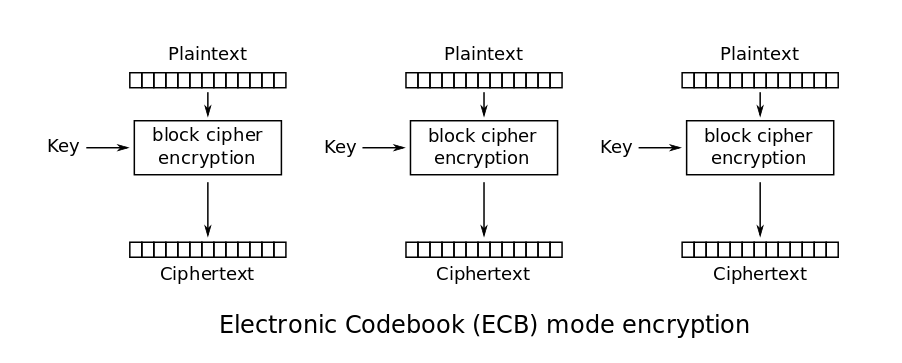
\includegraphics[width=0.47\linewidth]{./chapters/applications/mode-of-operation/ECB-ENC.png}}} \label{fig-ECB-ENC}
					\qquad
					\subfloat{{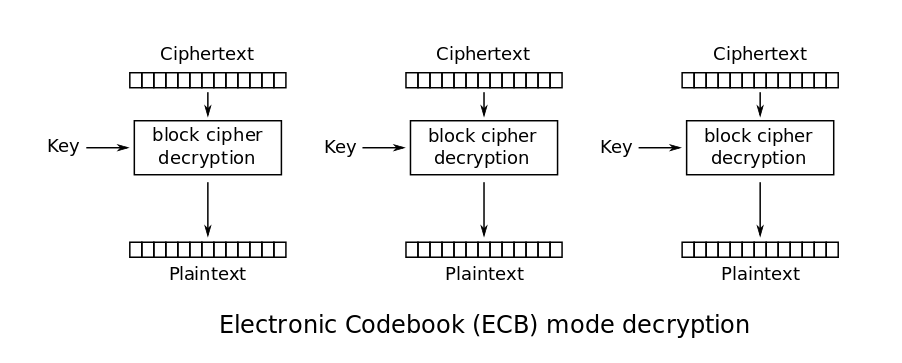
\includegraphics[width=0.47\linewidth]{./chapters/applications/mode-of-operation/ECB-DEC.png}}} \label{fig-ECB-DEC}
					\caption{ECB Mode}
					\label{fig-ECB}
				\end{figure}
				Since same plaintext blocks are encrypted into same ciphertext block, the blocks can be copied, or replayed, to change the message easily. This is called the \emph{Block Replay Attack}.

			\subsubsection{Cipher Block Chaining(CBC)}
				CBC takes the previous ciphertext block and XOR($\bigoplus$) it with the plaintext before encryption. The first block has no previous ciphertext block, hence it is XOR-ed with the $IV$. In equation:
				\begin{itemize}
					\item \textbf{Encryption} $C_0=IV$, $C_i=E_K(P_i \bigoplus C_{i-1}), i=1,2,3,\cdots,N$
					\item \textbf{Decryption} $C_0=IV$, $C_i=D_K(C_i) \bigoplus C_{i-1}, i=1,2,3,\cdots,N$
				\end{itemize}
				\begin{figure}[h!]
					\centering
					\subfloat{{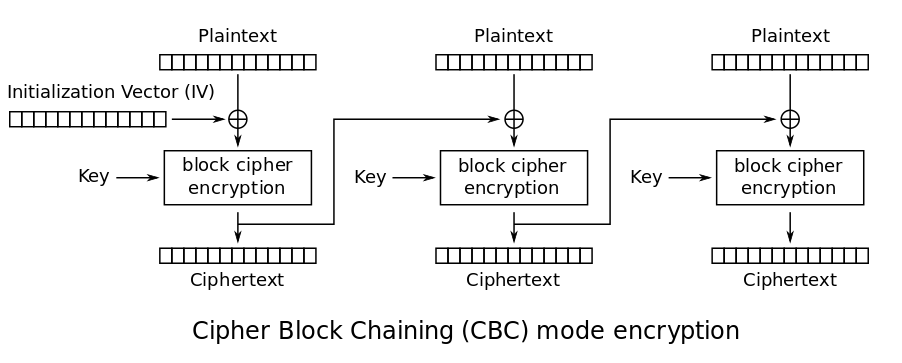
\includegraphics[width=0.47\linewidth]{./chapters/applications/mode-of-operation/CBC-ENC.png}}} \label{fig-CBC-ENC}
					\qquad
					\subfloat{{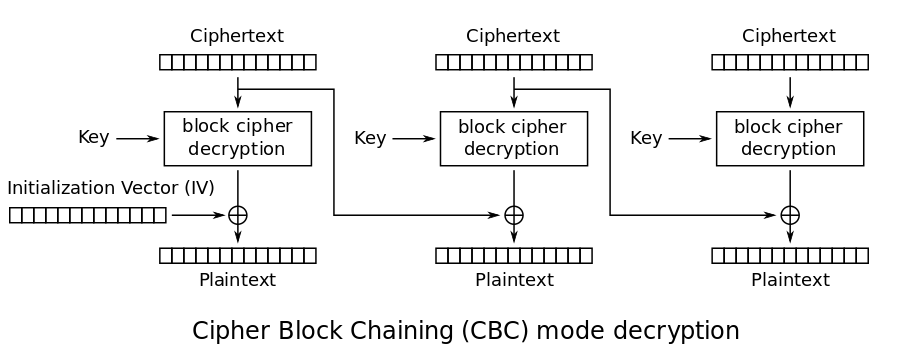
\includegraphics[width=0.47\linewidth]{./chapters/applications/mode-of-operation/CBC-DEC.png}}} \label{fig-CBC-DEC}
					\caption{CBC Mode}
					\label{fig-CBC}
				\end{figure}
			
			\subsubsection{Cipher Feedback(CFB)}
				CFB can be used to encrypt a block even smaller than the size of the encryption block, and can be used to make a stream cipher out of block cipher. In the diagram given below, original block sizes are used. In equation:
				\begin{itemize}
					\item \textbf{Encryption} $C_0=IV$, $C_i=E_K(P_i \bigoplus C_{i-1}), i=1,2,3,\cdots,N$
					\item \textbf{Decryption} $C_0=IV$, $C_i=D_K(C_i) \bigoplus C_{i-1}, i=1,2,3,\cdots,N$
				\end{itemize}
				\begin{figure}[h!]
					\centering
					\subfloat{{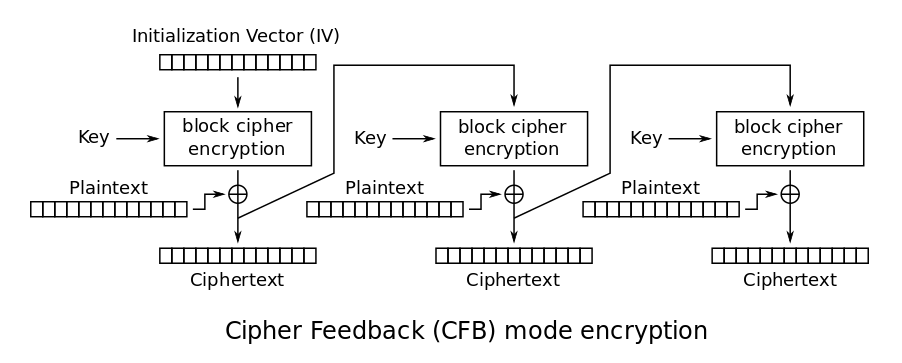
\includegraphics[width=0.47\linewidth]{./chapters/applications/mode-of-operation/CFB-ENC.png}}} \label{fig-CFB-ENC}
					\qquad
					\subfloat{{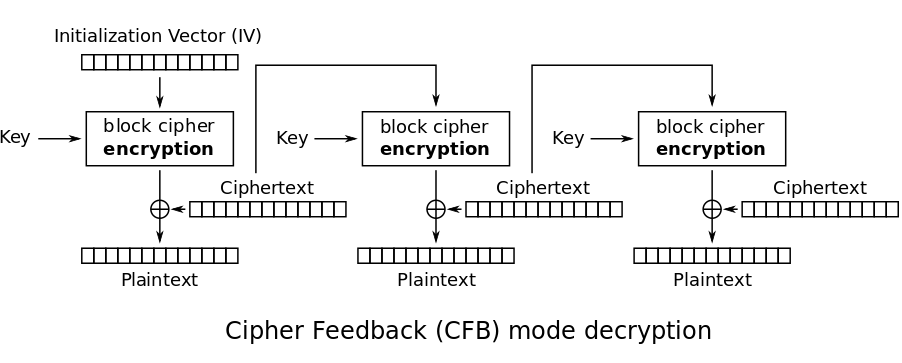
\includegraphics[width=0.47\linewidth]{./chapters/applications/mode-of-operation/CFB-DEC.png}}} \label{fig-CFB-DEC}
					\caption{CFB Mode}
					\label{fig-CFB}
				\end{figure}
				By altering the equation to the following we have the ``stream cipherized`` version, where $<<$ is the shift operation, $head(a,x)$ is the first $x$ bits of $a$, and $n$ is the size of the $IV$:
				\begin{itemize}
					\item \textbf{Shift Register} $S_0=IV$, $S_i=((S_i<<x)+C_i) \mod 2^n$
					\item \textbf{Encryption} $C_i=head(E_K(S_{i-1}),x) \bigoplus P_i$
					\item \textbf{Decryption} $P_i=head(E_K(S_{i-1}),x) \bigoplus C_i$
				\end{itemize}

			\subsubsection{Output Feedback(OFB)}
				OFB can be used to encrypt a block even smaller than the size of the encryption block, and can be used to make a stream cipher out of block cipher.
				\begin{itemize}
					\item \textbf{Input and Output} $I_0=IV$, $I_j=E_K(I_{j-1}), j=1,2,3,\cdots,N$
					\item \textbf{Encryption} $C_j=P_j \bigoplus I_j, i=1,2,3,\cdots,N$
					\item \textbf{Decryption} $P_j=C_j \bigoplus I_j, i=1,2,3,\cdots,N$
				\end{itemize}
				\begin{figure}[h!]
					\centering
					\subfloat{{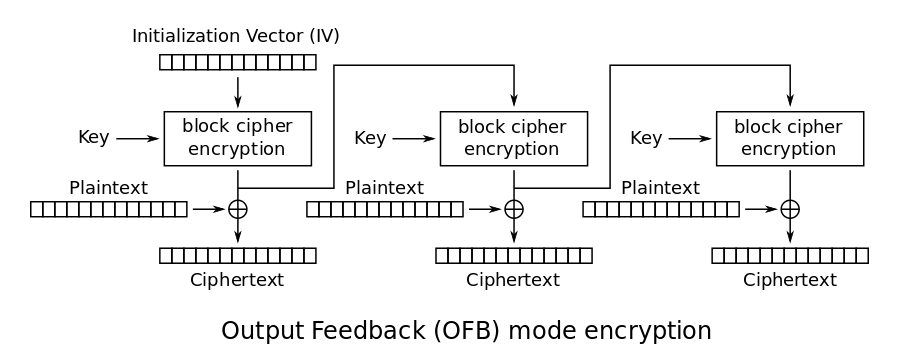
\includegraphics[width=0.47\linewidth]{./chapters/applications/mode-of-operation/OFB-ENC.png}}} \label{fig-OFB-ENC}
					\qquad
					\subfloat{{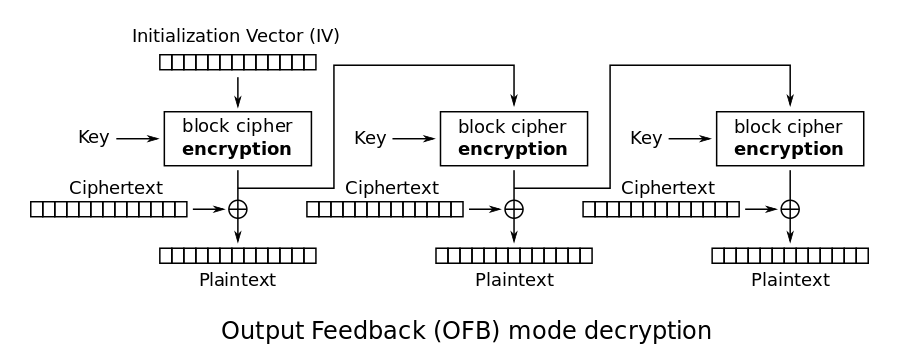
\includegraphics[width=0.47\linewidth]{./chapters/applications/mode-of-operation/OFB-DEC.png}}} \label{fig-OFB-DEC}
					\caption{OFB Mode}
					\label{fig-OFB}
				\end{figure}
				We can similarly alter the equation as OFB so that it can be used as a stream cipher.
			
			\subsubsection{Counter(CTR)}
				CTR can be used to encrypt a block even smaller than the size of the encryption block, and can be used to make a stream cipher out of block cipher. It encrypts the counter value instead of the plaintext, and XORs the value to gain the ciphertext.
				\begin{itemize}
					\item \textbf{Encryption} $C_i=P_i \bigoplus E_K(Counter), i=1,2,3,\cdots,N$
					\item \textbf{Decryption} $P_i=C_i \bigoplus E_K(Counter), i=1,2,3,\cdots,N$
				\end{itemize}
				\begin{figure}[h!]
					\centering
					\subfloat{{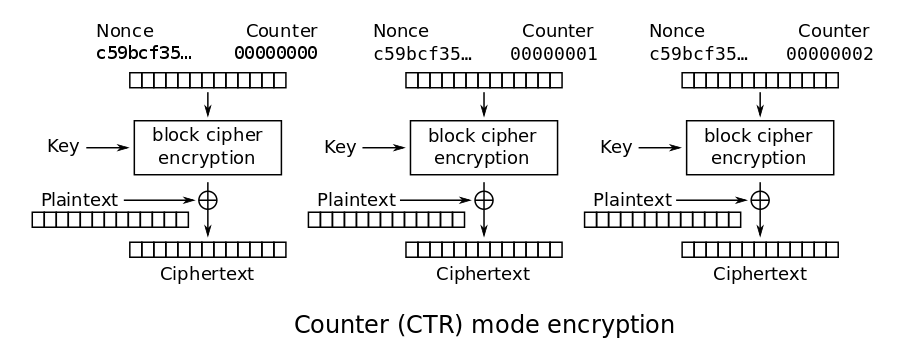
\includegraphics[width=0.47\linewidth]{./chapters/applications/mode-of-operation/CTR-ENC.png}}} \label{fig-CTR-ENC}
					\qquad
					\subfloat{{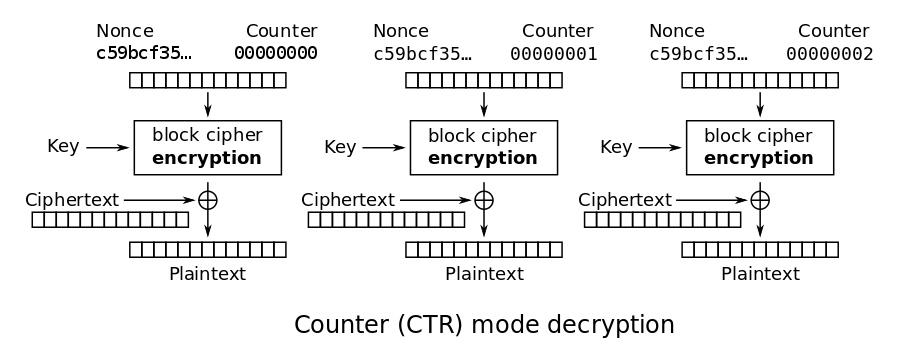
\includegraphics[width=0.47\linewidth]{./chapters/applications/mode-of-operation/CTR-DEC.png}}} \label{fig-CTR-DEC}
					\caption{CTR Mode}
					\label{fig-CTR}
				\end{figure}
				We can similarly alter the equation as OFB so that it can be used as a stream cipher.
			
				\subsubsection{Characteristics}
				Table \ref{table-mode-of-operation} shows the characteristics for each modes of operation.
				\begin{itemize}
					\item Block Pattern: Whether if the overall pattern is kept after encryption
					\item Preprocessing: Whether if preprocessing is possible on encryption and decryption
					\item Parallel Processing: Whether if parallel processing is possible on encryption or decryption
					\item Error Propagation: If there is an error in the encryption/decryption process, whether if the error spreads through other blocks
					\item Encryption Unit: The minimum requirement byte for encryption
				\end{itemize}
				\begin{table}[]
					\begin{tabular}{ccccccc}
						\multicolumn{2}{c}{}                              & ECB & CBC         & CFB         & OFB & CTR \\
						\multicolumn{2}{c}{Block Pattern}                 & O   & X           & X           & X   & X   \\
						\multicolumn{2}{c}{Preprocessing}                 & X   & X           & X           & O   & O   \\
						\multirow{2}{*}{Parallel Processing} & Encryption & O   & X           & X           & O   & O   \\
						& Decryption & O   & O           & O           & O   & O   \\
						\multicolumn{2}{c}{Error Propagation}             & X   & $(P_i,P_{i+1})$ & $\lceil \frac{n}{r} \rceil$ blocks & X   & X   \\
						\multicolumn{2}{c}{Encryption Unit}               & $n$   & $n$           & $r (\leq n)$           & $r (\leq n)$   & $r (\leq n)$  
					\end{tabular}
					\caption{Characteristics for Each Modes of Operation}
					\label{table-mode-of-operation}
				\end{table}
			
	\section{Types of Attack}
		\subsection{Attacking Classical Cryptosystems} 
			Classical Cryptosystems are typically a substitution cipher and/or a transposition cipher. Since most, if not all, the classical cryptosystems are broken, the two valid ways to attack any classical cryptosystems is given here.
			\begin{itemize}
				\item Brute Force Attack
				\subitem When the attacker gains the ciphertext $c$, the attacker uses every key possibility to try to gain $m$. This is otherwise known as the Exhaustive Key Search Attack. Theoretically this can be done to any symmetric-key cipher; but this is inapplicable to most modern cryptosystems as they have an extremely large key space.
				
				\item Frequency Analysis
				\subitem The plaintext having some pattern, such as the alphabet `e` appearing with the most frequency, will help the attacker gain knowledge on the plaintext just by seeing the ciphertext.
			\end{itemize}
		
	\section{Cryptographic Hash Functions}
		A general hash function has the following properties:
		\begin{itemize}
			\item They take an arbitrary size of data as input, and;
			\item They produce a constant and fixed length data as output.
		\end{itemize}
		A \emph{cryptographic hash function}, in addition to the properties above, must have the following properties:
		\begin{itemize}
			\item Preimage Resistance
			\subitem If the hash value $y$ is given, it must be hard to find an $x$ such that $h(x)=y$, that is, the hash function must have one-wayness.
			\item Second Preimage Resistance
			\subitem If the message $x$ is given, it must be hard to find an $x' \ne x$ such that $h(x)=h(x')$.
			\item Collision Resistance
			\subitem It must be hard to find $x \ne x'$ such that $h(x)=h(x')$. The pair $(x,x')$ is called the collision pair.
		\end{itemize}
		
	\section{Attacking the Cyrptosystems}
		Attacks on cryptosystems are classified into \emph{passive} and \emph{active} attack.
		Passive attacks simply eavesdrops the transmission, and gains what the attacker wants without modification of the message. This type of attacking includes \emph{eavesdropping}, of which the attacker intercepts the message in the middle to check the plaintext. This type of attacker is often referred to as "Eve"(as in eavesdropping) in theories.
		Active attackers will modify the message, which includes Modification, Deletion, Impersonation, and Replay. This type of attacker can also be referred to as "Eve", but sometimes is referred to as "Mallory", for malicious user.
		\begin{itemize}
			\item Modification: Changes the order of the message or changes a part of it to alter the meaning.
			\item Deletion: Intercepts the message and does not send it, interrupting the communication.
			\item Impersonation: Fakes their own identity to be identified as a correct user.
			\item Replay: Send a message again after eavesdropping, expecting some kind of result.
		\end{itemize}
		The four methods above are just the general ways to attack. We need to attack the system itself to know how to attack it. There are four methods of attack on system:
		\begin{itemize}
			\item \textbf{Ciphertext Only Attack}
			\subitem The attacker knows only the ciphertext.
			\item \textbf{Known Plaintext Attack}
			\subitem The attacker knows a list of (message, ciphertext) pair, and attempts to crack a ciphertext not in the list.
			\item \textbf{Chosen Plaintext Attack}
			\subitem The attacker has access to an oracle that can encrypt the message, and attempts to crack a ciphertext.
			\item \textbf{Chosen Ciphertext Attack}
			\subitem The attacker has access to an oracle that can decrypt a ciphertext, except for the target ciphertext.
		\end{itemize}
		There are three important properties to encryption schemes:
		\begin{itemize}
			\item Semantic Security
			\subitem A semantically secure encryption scheme is infeasible for any computationally bounded adversary to derive a significant information about the original plaintext when given only its ciphertext and the corresponding public key if any. This can be represented as a game between the oracle and the adversary, as below:
			\begin{enumerate}
				\item The oracle generates a key for the challenge.
				\item The adversary is given the encryption oracle(or the public key, in the case of public key cryptosystem).
				\item The adversary can perform any number of polynomially bounded number of encryptions or operations.
				\item The adversary generates two equal-length messages $m_0$ and $m_1$, and transmits it to the oracle.
				\item The oracle randomly chooses $b \in \{0,1\}$ to encrypt the message $m_b$ to $C$.
				\item The adversary, upon receiving $C$, guesses $b$.
			\end{enumerate}
			If the adversary cannot guess $b$ correctly with significantly greater than 50\% probability, then the scheme is said to be semantically secure under CPA.
			
			\item Indistinguishability
			\subitem If a cryptosystem is indistinguishable, then an adversary would not be able to distinguish pairs of ciphertexts based on the message they encrypt. There are three types: IND-CPA, IND-CCA1, and IND-CCA2. They can be represented as a game between the oracle and the adversary. In both cases, they are said to be secure if the adversary does not have a clear advantage.
			\begin{itemize}
				\item \textbf{IND-CPA}
				\begin{enumerate}
					\item The oracle generates a key for the challenge.
					\item The adversary is given the encryption oracle(or the public key, in the case of public key cryptosystem).
					\item The adversary can perform any number of polynomially bounded number of encryptions or operations.
					\item The adversary generates two distinct equal-length messages $m_0$ and $m_1$, and transmits it to the oracle.
					\item The oracle randomly chooses $b \in \{0,1\}$ to encrypt the message $m_b$ to $C$.
					\item The adversary, upon receiving $C$, performs polynomially bounded encryptions or operations, and guesses $b$.
				\end{enumerate}
				\item \textbf{IND-CCA}
				\begin{enumerate}
					\item The oracle generates a key for the challenge.
					\item The adversary is given the decryption oracle and the public key, in the case of public key cryptosystem.
						\subitem Note that in the case of the public key cryptosystem, the encryption oracle is also given.
					\item The adversary can perform any number of polynomially bounded number of decryptions or operations.
					\item The adversary generates two distinct equal-length messages $m_0$ and $m_1$, and tramsmits it to the oracle.
					\item The oracle randomly chooses $b \in \{0,1\}$ to encrypt the message $m_b$ to $C$.
					\item The adversary, upon receiving $C$, performs polynomially bounded operations.
						\subitem In the case of IND-CCA1, the adversary may not make further calls to the decryption oracle.
						\subitem In the case of IND-CCA2, the adversary may make further calls to the decryption oracle, but may not submit $C$.
					\item The adversary guesses $b$.
				\end{enumerate}
			\end{itemize}
			This can be said with a random oracle. In that case, the adversary submits only one message and the oracle returns the encryption of the message or the random string equal to the length of the encryption with a fair chance. The adversary then guesses whether if the message is randomly generated or encrypted.

			\item Non-malleability
			\subitem Cryptosystems are called "malleable" if it is possible to transform a ciphertext into another ciphertext which decrypts to a related plaintext. Cryptosystems that are not malleable are called non-malleable. These, similar to indistinguishability, can be represented as a game between the oracle and the adversary, and are called NM-CPA, NM-CCA1, NM-CCA2.
		\end{itemize}
	
		\begin{thm}
			The following relations for each security properties hold:
			\begin{itemize}
				\item IND-CPA $\Leftrightarrow$ Semantic security under CPA
				\item NM-CPA $\Rightarrow$ IND-CPA
				\item NM-CCA2 $\Leftrightarrow$ IND-CCA2
				\item NM-CPA  does not necessarily imply IND-CCA2.
			\end{itemize}
		\end{thm}
		
	\section{Digital Signatures}
		Digital signatures are used in pair with the public key cryptosystems to verify the sender of the messages. When attacking, there are three major methods:
		\begin{itemize}
			\item \textbf{Key-Only Attack}
			\subitem The attacker only has access to the digital signature algorithm and the public key of the signer, $pk_A$. This is similar to the Ciphertext Only attack.
			\item \textbf{Known Message Attack}
			\subitem The attacker has access to the digital signature algorithm, the public key of the signer, and a list of (message, signature) pairs. This is similar to the Known Plaintext attack.
			\item \textbf{Chosen Message Attack}
			\subitem The attacker has access to the digital signature algorithm, the public key of the signer, and an oracle that takes a message as an input and returns signature as an output.
		\end{itemize}
		The attacker can have three different purposes:
		\begin{itemize}
			\item \textbf{Total Break}
			\subitem The attacker wants to gain the private key of the signer.
			\item \textbf{Selective Forgery}
			\subitem The attacker wants to generate a valid signature for a message the attacker wants(i.e. any message for that matter).
			\item \textbf{Existential Forgery}
			\subitem The attacker wants to generate a valid (message, signature) pair for any message.
		\end{itemize}
		It is said that an attack is valid if the attack succeeds with a non-negligible probability.
		
	\section{Zero-Knowledge Authentication}
		Three major ways to authenticate a user is using password, challenge-response, and zero-knowledge authentication. Passwords must be sent through network, thereby they are susceptible to interception. Challenge-response can be abused by malicious users to crack the secret key. That is where the concept of zero-knowledge interactive proof comes in.
		
		An interactive proof system can be described as a communication between the verifier and the prover. They exchange messages to check whether if the statement is true or false. In here, the prover is assumed to have unlimited calculating power but cannot be trusted; the verifier has bounded computation power but is assumed to be always honest. Messages are sent between the prover and the verifier until the verifier has an answer to the problem and has convinces itself that the answer is correct.
		Any interactive proof system must have the following properties:
		\begin{itemize}
			\item \textbf{Completeness}: If the statement is true, the honest verifier will be convinced of this fact by an honest prover.
			\item \textbf{Soundness}: If the statement is false, no cheating prover can convince the honest verifier that it is true, except with some small probability.
		\end{itemize}
		In authentication, if the proof is only interactive, a malicious verifier may abuse the protocol to reveal the ``knowledge``(in the case for cryptosystems, private keys) only the prover knows. This is where the concept of ``Zero-knowledgeness`` comes in.
		\begin{itemize}
			\item \textbf{Zero-knowledgeness}: If the statement is true, no verifier can learn anything apart from the fact that the statement is true.
		\end{itemize}
		The best way to describe this is by an analogy of a colorblind person. Suppose the person has two balls that looks the exactly same for them. Their friend, as a non-colorblind person, want to prove that the two balls are of different color. The colorblind person resumes the role of verifier and the non-colorblind friend the prover. Here is an example protocol on how the fact can be proven:
		\begin{enumerate}
			\item Verifier shows you a ball.
			\item Prover memorize it.
			\item Verifier then hides both balls, and choose to keep the ball shown before or change the ball.
			\item Verifier shows the newly chosen ball.
			\item Prover tell verifier whether if the ball has been changed or not.
			\item If the prover is wrong, the prover has told a lie; end the protocol.
			\item If the prover is right, the prover may be telling the truth; continue the protocol until convinced.
		\end{enumerate}
		If the statement(`The two balls are of different color`) is false, then the prover(in this case, cheating) cannot tell whether if the ball has been changed; therefore their guess is right for 50\% of the time. $n$ consecutive application of the protocol gives $\frac{1}{2^n}$ chance of success, and as the number of trials increase, the less the cheating prover will be able to pass the protocol.
		
		If the statement, on the other hand, is indeed true, then the prover can tell whether if the ball has been switched every time. In the verifier's point of view, the prover's $n$-th consecutive success for verification proves that they are lying at $\frac{1}{2^n}$ probability; their improbable probability of success at lying will thereby prove their honesty.
		
	\section{RSA Cryptosystem and Signature}
		\subsection{Keygen}
		\begin{enumerate}
			\item Choose two primes $p$ and $q$.
			\item Let $n=p\cdot q$.
			\item Choose $e$ such that $(e,\phi(n))=1$
			\item Find $d$ such that $e\cdot d\equiv 1 \mod \phi(n)$
		\end{enumerate}
		\textbf{Public Key}: $(n,e)$\\
		\textbf{Private Key}: $d$ or $(p,q,d)$, depending on the method.
		
		\subsection{Cryptosystem}
			\subsubsection{Encryption}
			$C\equiv M^e \mod n$
			
			\subsubsection{Decryption}
			\begin{itemize}
				\item \textbf{Basic Method}\\
				$C^d \equiv (M^e)^d \equiv M^{\phi(n)\cdot k+1}\equiv M \mod n$
				\item \textbf{Chinese Remainder Theorem}\\
				Split $C^d \mod n$ into two congruences: $C^d \mod p$ and $C^d \mod q$.\\
				Using Euler's Theorem(If $(a,n)=1$, $a^{\phi(n)} \mod n$.), reduce $d$ to reduce the number of multiplication.
			\end{itemize}
		
		\subsection{Signature}
			\subsubsection{Signing}
			$S \equiv M^d \mod n$
			
			\subsubsection{Verifying}
			Compare $S^e \mod n$ to $M$. If equal, accept; otherwise reject.
		
		\subsection{Attacking the Cryptosystem}
			\subsubsection{On the Case of Exposed Private Key $e$}
			For the public key, $n=pq$ where $p$ and $q$ are primes.\\
			Then, $\phi(n)=(p-1)(q-1)$.\\
			We know that $ed \equiv 1 \mod \phi(n)$.\\
			By the definition of modular, $ed-1=k \phi(n)$ for some $k$.\\
			For a large enough $n=pq$, $\frac{\phi(n)}{n} = \frac{(p-1)(q-1)}{pq} = 1 - \frac{1}{p} - \frac{1}{q} +\frac{1}{pq}  \simeq 1$.\\
			We can find $k$ by dividing both sides of the equation $ed-1=k \phi(n)$ by $n$, since $\frac{ed-1}{n}=k\frac{\phi(n)}{n} \simeq k$.\\
			We can then find $\phi(n)=\frac{ed-1}{k}$.\\
			Since $n=pq$ and $\phi(n)=(p-1)(q-1)=pq-(p+q)+1=n-(p+q)+1$, $p+q=n-\phi(n)+1$.\\
			Then the quadratic equation $(x-p)(x-q)=x^2-(p+q)x+pq=x^2-(n-\phi(n)+1)x+n=0$ can be solved to yield $p$ and $q$.
			
			\subsubsection{Chosen Ciphertext Attack}
			\begin{enumerate}
				\item Alice sends $C\equiv M^e \mod n$ to Bob
				\item Eve intercepts Alice's transmission; chooses $x$ s.t. $(x,n)=1$(and therefore $x^{-1} \mod n$ exists) to send $C'=Cx^e \mod n$ to Bob.
				\item Bob decrypts $C'$ as $(C')^d \equiv (Cx^e)^d \equiv C^d x^{ed} \equiv Mx \mod n$
				\item Eve intercepts Bob's decryption result, $Mx$, and multiplies $x^{-1}$ modulo $n$ to gain $M$.
			\end{enumerate}
			
			\subsubsection{Coppersmith Attack} \label{coppersmith-attack}
			\begin{thm}[Coppersmith]
				Let $n \in \mathbb{Z}$ and $f \in \mathbb{Z}[x]$ be a monic polynomial(i.e. leading coefficient of $f$ is $1$) of degree $d$ over integer.\\
				Set $X=n^{1/d-\epsilon}$ for $1/d>epsilon>0$.
				Then given $n$ and $f$, the attacker, using the \href{https://en.wikipedia.org/wiki/Lenstra\%E2\%80\%93Lenstra\%E2\%80\%93Lov\%C3\%A1sz_lattice_basis_reduction_algorithm}{LLL Algorithm}, can efficiently find all integer $x_0<X$ such that $f(x_0) \equiv 0 \mod n$.
			\end{thm}
			\begin{note}
				In the case of RSA, Finding $M$ when given $C \equiv M^e \mod n$ can be interpreted as finding the solution of the equation $f(x) \equiv x^e - C \mod n$. This attack's strength is the ability to find all small roots of the polynomials modulo a composite $N$.
			\end{note}
			
			\subsubsection{Håstad's Broadcast Attack}
			This attack is viable if the value of $e$ is fixed and is small, and the same message is broadcast without padding.
			
			Suppose the same plaintext $M$ is encrypted to multiple people, each using same $e$ and different moduli, say $N_i$. If Eve successfully intercepts $e$ or more messages, say $C_1,C_2,\cdots,C_e$, $C_i \equiv M^e \mod N_i$. We may assume $(N_i,N_j)=1$ for $i \ne j$, otherwise the attacker will be able to factorize some $N_i$ by finding their GCD. Using the Chinese Remainder Theorem on the $e$ congruences, the attacker may compute $C \in Z_{\Pi N_i}^*$ such that $C_i \equiv C \mod N_i$. Then, $C \equiv M^e \mod \Pi N_i$; however since $M<N_i$ for each $i$, $M^e<\Pi N_i$; thus $C=M^e$ holds over the integers, and the attacker can easily find the message $M$.
			
			For more generalized version, the following theorem is available:
			\begin{thm}[Håstad]
				Suppose $N_1,\cdots,N_k$ are relatively prime integers and set $N_{\min}=\min_i\{N_i\}$. Let $g_i(x) \in \mathbb{Z}/N_i[x]$ be $k$ polynomials of maximum degree $q$. Suppose there exists a unique $M<N_{\min}$ satisfying $g_i(M) \equiv 0 \mod N_i \forall i \in \{1,\cdots,k\}$. Furthermore, suppose $k>q$. Then there is an efficient algorithm which, given $\left< N_i,g_i(x)\right> \forall i$, computes $M$.
			\end{thm}
			This theorem can be used in the following way:\\
			Suppose the $i$-th plaintext is padded with the polynomial $f_i(x)$. Let $g_i(x)=(f_i(x))^{e_i}-C_i \mod N_i$. Then $g_i(M) \equiv 0 \mod N_i$ is true, and the Coppersmith's Attack[\ref{coppersmith-attack}] can be used.
			
			\subsubsection{Franklin-Reiter Related Message Attack}
			This attack is viable if the value of $e$ is fixed and is small, and the same message is broadcast with padding.
			
			\begin{thm}
				Let $(n,e)$ be the public key of RSA, and $e$ is small.
				Let $f(x)=ax+b \in Z_n[x]$, $b \ne 0$; i.e. $f$ is the padding function.\\
				Suppose that $M_1 \ne M_2$ and $M_1 \equiv f(M_2) \mod n$.\\
				Then, given the quintuplet $(n,e,C_1,C_2,f)$, $M_1$ and $M_2$ can be recovered in $O((log_2n)^2)$
			\end{thm}
			
			\begin{proof}
				\begin{math}
				\\
				C_1 \equiv M_1^e \mod n\\
				C_2 \equiv M_2^e \mod n\\
				M_1 \equiv f(M_2) \equiv aM_2+b \mod n\\
				\\
				\text{Let } g_2(x)=x^e-C_2 \mod n \text{, and } g_1(x)=(ax+b)^e-C_1 \mod n\\
				\\
				g_1(x)=(ax+b)^e-C_1\\
				=(ax+b)^e-M_1^e\\
				=(ax+b)^e-(aM_2+b)^e\\
				=((ax+b)-(aM_2+b))Q(x)\\
				=a(x-M_2)Q(x)\\
				\\
				g_2(x)=x^e-C_2\\
				=x^e-M_2^e\\
				=(x-M_2)Q'(x)\\
				\\
				\rightarrow (x-M_2)|(g_1(x),g_2(x)\\
				\end{math}
				Using the euclidean algorithm on the two polynomials $g_1$ and $g_2$, $M_2$ can be recovered.
			\end{proof}
		
		\subsection{Forgeries of the Signature}
			\subsubsection{Known Message Attack}
			Suppose $(M_1,S_1)$ and $(M_2,S_2)$ are both valid signatures.\\
			Then, $(M_1M_2,S_1S_2)$ is also a valid signature.
			
			\subsubsection{Chosen Message Attack}
			Eve chooses $M_1$ and $M_2$ s.t. $M=M_1M_2$.\\
			Eve asks Alice to sign $M_1$ and $M_2$; let them be $S_1$ and $S_2$.\\
			Then $S_1S_2$ is a valid signature for $M$.
		
	\section{ElGamal Cryptosystem}
		\subsection{Keygen}
			Choose a prime $p$. Note that $(Z_p^*,\times)$ is a cyclic group.
			\begin{itemize}
				\item Choose $e_1$ to be the primitive root of $(Z_p^*,\times)$
				\item Choose $d \in Z_p^*$ and compute $e_2 \equiv e_1^d \mod p$
			\end{itemize}
			In theory, $p$ and $e_1$ can be shared as long as $e_2$ are kept distinct.
			\textbf{Public Key}: $(e_1,e_2,p)$\\
			\textbf{Private Key}: $d$
		
		\subsection{Cryptosystem}
			\subsubsection{Encryption}
				Randomly choose $r \in Z_p^*$. $M$ is the message.
				\begin{itemize}
					\item $C_1 \equiv e_1^r \mod p$
					\item $C_2 \equiv Me_2^r \mod p$
				\end{itemize}
				\textbf{Ciphertext}: $(C_1,C_2)$
			
			\subsubsection{Decryption}
				$C_2(C_1^d)^{-1} \equiv Me_2^r(e_1^{rd})^{-1} \equiv M(e_1^d)^r(e_1^{rd})^{-1} \equiv M \mod p$
		
		\subsection{Signature}
			\subsubsection{Signing}
				Randomly choose $r \in Z_p^*$. $M$ is the message.
				\begin{itemize}
					\item $S_1 \equiv e_1^r \mod p$
					\item $S_2 \equiv (M-dS_1)r^{-1} \mod (p-1)$
				\end{itemize}
				\textbf{Signature}: $(S_1,S_2)$
			
			\subsubsection{Verifying}
				Calculate:
				\begin{itemize}
					\item $V_1 \equiv e_1^M \mod p$
					\item $V_2 \equiv e_2^{S_1}S_1^{S_2} \mod p$
				\end{itemize}
				Verify with:
				\begin{itemize}
					\item Check $0<S_1<p$, $0<S_2<p-1$.
					\item Check $V_1=V_2$
				\end{itemize}
				\begin{math}
				V_2 \equiv e_2^{S_1}S_1^{S_2} \equiv (e_1^d)^{S_1}(e_1^r)^{S_2} \equiv e_1^{dS_1+rS_2} \equiv e_1^M \equiv V_1 \mod p
				\end{math}
		
		\subsection{Attacking the Cryptosystem}
			\subsubsection{Exposure of $r$}
				Since $(C_1,C_2)$ and $r$ are exposed, $M=C_2(e_2^r)^{-1} \mod p$.
			
			\subsubsection{Baby step, Giant step}
				When the random number $r$ is small, then the following meet-in-the-middle attack is possible:\\
				$y=e_1^x \mod p$.\\
				Let $m= \lceil \sqrt{p} \rceil$.\\
				Then, $\exists q,r \in \mathbb{Z}$ such that $x=mq+r, 0 \le r \le m-1$\\
				$\Rightarrow y=e_1^x \equiv e_1^{mq+r} \mod p$\\
				$\Rightarrow y(e_1^{-m})^q \equiv g^r \mod p$\\
				Hence we can find $r$ using the following protocol:
				\begin{enumerate}
					\item Construct the table with entries $(r,e_1^r \mod p), 0 \le r \le m-1$: (Baby step table)
					\item Compute the value $g^{-m} \mod p$: (Giant step value)
					\item For $q$ from $0$ to $m-1$, find $q$ such that $y(g^{-m})^q \equiv g^r \mod p$ in the table.
				\end{enumerate}
			
			\subsubsection{Known Plaintext Attack}
				Suppose the random number $r$ is reused to encrypt two distinct messages, $M$ and $M'$.\\
				Suppose $M$ encrypted to $(C_1,C_2)$; $M'$ encrypted to $(C_1',C_2')$.\\
				Note that $C_1=C_1'=e_1^r$, $C_2=Me_2^r$, $C_2'=M'e_2^r$.\\
				If we know $M'$, then $\frac{C_2\times M'}{C_2'}=\frac{Me_2^r\times M'}{M'e_2^r}=M$
		
		\subsection{Forgeries of the Signature}
			\subsubsection{Constructing from Scratch: One Variable}
				Choose $1<x<p-1$.
				\begin{itemize}
					\item $S_1 \equiv e_1^xe_2 \mod p$
					\item $S_2 \equiv -S_1 \mod (p-1)$
					\item $M \equiv xS_2 \mod (p-1)$
				\end{itemize}
			
			\subsubsection{Constructing from Scratch: Two Variables}
				Choose $u,v\in Z_p^*$ such that $(v,p-1)=1$ so that $\exists v^{-1} \mod(p-1)$
				\begin{itemize}
					\item $S_1 \equiv e_1^ue_2^v \mod p$
					\item $S_2 \equiv -S_1v^{-1} \mod (p-1)$
					\item $M \equiv S_2u \mod(p-1)$
				\end{itemize}
		
			\subsubsection{Known Plaintext Attack}
				A valid signature $(M,(S_1,S_2))$ is given for $(M,p-1)=1$ so that  $\exists M^{-1} \mod (p-1)$.\\
				Choose a message $M'$.\\
				Set $u=M'M^{-1} \mod (p-1)$.\\
				Compute $S_2 \equiv S_2u \mod (p-1)$.\\
				Solve the following set of linear congruences using CRT:
				\begin{displaymath}
				\begin{cases}
				S_1'=S_1u \mod(p-1)\\
				S_1'=S_1 \mod p
				\end{cases}
				\end{displaymath}
				Then, $(M',(S_1',S_2'))$ is also a valid signature, if the range conditions are not checked.
		
	\section{Schnorr Digital Signature}
		Signatures based on cryptosystems have a weakness: they pose a threat to expose the secret key, or makes it easier to forge a specific message. Schnorr Digital Signature is a signature-only algorithm that helps solve this.
		\subsection{Keygen}
			\begin{itemize}
				\item Choose a cryptographic hash function $h$.
				\item Choose a prime $p$.
				\item Choose a prime $q$ such that:
					\subitem $q|p-1$, and;
					\subitem The size of $q$ is the same as the hash output.
				\item Choose $e_0$ such that it is a generator in $Z_p^*$.
				\item Set $e_1 \equiv e_0^{(p-1)/q} \not\equiv 1 \mod p$.
				\item Choose $d$.
				\item Set $e_2 \equiv e_1^d \mod p$.
			\end{itemize}
			\textbf{Public Key}: $(h,e_1,e_2,p,q)$\\
			\textbf{Private Key}: $d$

		\subsection{Signature}
			\subsubsection{Signing}
				Choose $r \in Z_q^*$ at random.
				\begin{itemize}
					\item $S_1=h(M||e_1^r \mod p)$ where $||$ is concatenation.
					\item $S_2=r+dS_1 \mod q$
				\end{itemize}
				\textbf{Signature}: $(S_1,S_2)$
			
			\subsubsection{Verifying}
				Calculate $V=h(M||e_1^{S_2}e_2^{-S_1} \mod p)$.\\
				If $V=S_1$, then $M$ is accepted.\\
				\begin{math}
					e_1^{S_2}e_2^{-S_1}=e_1^{r+dS_1}e_1^{-dS_1}=e_1^r \mod p
				\end{math}
\end{document}

\end{document}